\documentclass{article}
\usepackage{blindtext}
\usepackage{titlesec}
\usepackage{listings}
\usepackage{geometry}
\usepackage{mathtools}
\usepackage[utf8]{inputenc}
\usepackage{siunitx}
\usepackage{soul}
\usepackage{enumitem}
\usepackage{graphicx}
\usepackage{float}
\usepackage{units}
\usepackage{amsfonts}
\usepackage{graphicx}
\usepackage{amsfonts,amssymb,amsmath,hyperref}
\usepackage{color}
\usepackage{tcolorbox}
\usepackage[bottom]{footmisc}

\geometry{
 a4paper,
 total={170mm,257mm},
 left=20mm,
 top=20mm,
 }
 
\setlength{\parindent}{0pt}

\title{Real-Time Digital Signal Processing}

\author{
  Pranav Malhotra, CID:\num{00823617}
}
\date{2nd February 2016}

\definecolor{codegreen}{rgb}{0.1,0.5,0.1}
\definecolor{codegray}{rgb}{0.5,0.5,0.5}
\definecolor{codepurple}{rgb}{0.58,0,0.82}
\definecolor{backcolour}{rgb}{1,1,1}
\definecolor{codemaroon}{rgb}{0.5,0,0}

\lstdefinestyle{mystyle}{
    backgroundcolor=\color{backcolour},   
    commentstyle=\color{codegreen},
    keywordstyle=\color{codemaroon},
    numberstyle=\tiny\color{codegray},
    stringstyle=\color{codepurple},
    basicstyle=\footnotesize,
    breakatwhitespace=false,         
    breaklines=true,                 
    captionpos=b,                    
    keepspaces=true,                 
    numbers=left,                    
    numbersep=5pt,                  
    showspaces=false,                
    showstringspaces=false,
    showtabs=false,                  
    tabsize=2
}

\lstset{style=mystyle}



\title{Real-Time Digital Signal Processing Report 2}
\author{pranav.malhotra13 }
\date{February 2016}

\begin{document}

\begin{titlepage}
	\centering
	{\scshape\LARGE Imperial College London \par}
	\vspace{2cm}
	{\scshape\Large Real-Time Digital Signal Processing \par}
	\vspace{1cm}
	{\scshape\Large Laboratory 3\par}
	\vspace{2.5cm}
	{\Large\itshape Ahmad Moniri, CID: 00842685 \par}
	\vspace{1cm}
	{\Large\itshape Pranav Malhotra, CID: 00823617 \par}
	\vfill
% Bottom of the page
	\begin{tcolorbox}
    \centering
    Declaration: We confirm that this submission is our own work. In it, we give references and citations whenever we refer to or use the published, or
    unpublished, work of others. We are aware that this course is bound by
    penalties as set out in the College examination offences policy \\~\\
    \underline{Signed: Ahmad Moniri, Pranav Malhotra}
    \end{tcolorbox}
	{\large \today\par}
\end{titlepage}

\tableofcontents

\newpage
\section{Introduction}
In laboratory 2, the polling technique of communicating with peripherals was explored. When polling a peripheral, the processor cannot execute any other instruction and this presents a stark limitation on the usefulness of polled I/O software. In laboratory 3, interrupt-driven programming is introduced. Interrupt-driven programs are more efficient; such programs have the capacity to fully utilise the computation power of the processor/embedded device.\\

This report starts off by introducing the hardware that enables interrupt-driven programming. Following this, an in-depth discussion of the laboratory experiment is presented. This discussion includes a mathematical description of a fully rectified sine wave and aliasing and its effects. All theory is corroborated through experimental results that are presented in the form of scope traces.   

\section{Interrupt Service Routines}\label{sec:interrupt_service_routines}
A processor can communicate with multiple peripherals simultaneously. At any time, any one of these peripherals may need to send/receive data from the processor; when this happens, the peripheral raises a flag to signal that it needs servicing. De-conflicting interrupt requests (IRQs) is done on a dedicated piece of hardware called the interrupt handler. Each peripheral is allocated an interrupt priority; interrupts with higher priority are the first to be serviced. The interrupt handler contains a vector of addresses corresponding to the locations in memory where the code that services the specific interrupt is stored. \\

The interrupt handler will send this memory address to the processor's Program Counter (PC). An essential part of servicing interrupts is to ensure that the registers that the CPU is currently using are not corrupted. Thus, before the processor branches to a specific memory location, to service the interrupt, it performs a context save. This saves the current state of the registers that the Interrupt Service Routine (ISR) makes use of, on the stack. Once the ISR is completed, the state of the registers is restored. In many architectures, interrupts are classed into fast interrupts and slow interrupts. Fast interrupts contain additional hardware in the form of shadow registers that enable servicing of interrupts without the need for context saves. This can have a significant impact on the efficiency of the program if the interrupt needs to be serviced often. Mouse or keyboard actions are examples of events that may be assigned as fast interrupts.\\

The TMS320C6713 contains multiple on-chip peripherals. Texas Instrument provides Chip Support Libraries (CSLs) presenting the programmer an additional layer of abstraction that allows simple and effective communication with the on-chip peripherals. The AIC23 audio codec is not a simple memory-mapped peripheral and thus the Multi-Channel Buffered Serial Port (McBSP), which is an on-chip peripheral, is used to communicate with the it. The communication makes use of two serial ports; one uni-directional port is used to program the configuration registers in the audio codec, and one bi-directional port is used for data flows. \\

\textbf{It is of great importance to note that it is the MsBSPs that raise the IRQ and not the audio codec. CSL modules are used to deal with interrupts generated by the MsBSPs.}\\

\newpage
\section{Exercise 1}

\subsection{Hardware Initialisation}

Before programs are run on the DSK board, initialising the hardware to the required settings is necessary. The function {\tt init\textunderscore hardware} performs this operation. As noted in section \ref{sec:interrupt_service_routines}, the MsBSP needs to be connected to the AIC23 audio codec. This is achieved in line $11$ of the listing \ref{lst:init_hardware_pranav}. Following this, line $15$ serves to define the event that raises the IRQ: the acquisition of a 32 bit word from the AIC23 audio codec. It is also clear that 2 serial ports need to be initialised; one for configuration and one for data flows.\\

\begin{lstlisting}[language=C, frame=single, caption=Hardware Initialisation Settings, label = lst:init_hardware_pranav]
void init_hardware(){
    // Initialise the board support library, must be called first 
    DSK6713_init();

    // Start the AIC23 codec using the settings defined above in config 
    H_Codec = DSK6713_AIC23_openCodec(0, &Config);

    /* Function below sets the number of bits in word used by MSBSP (serial port) for 
    receives from AIC23 (audio port). We are using a 32 bit packet containing two 
    16 bit numbers hence 32BIT is set for  receive */
    MCBSP_FSETS(RCR1, RWDLEN1, 32BIT);	

    /* Configures interrupt to activate on each consecutive available 32 bits 
    from Audio port hence an interrupt is generated for each L & R sample pair */	
    MCBSP_FSETS(SPCR1, RINTM, FRM);

    /* These commands do the same thing as above but applied to data transfers to  
    the audio port */
    MCBSP_FSETS(XCR1, XWDLEN1, 32BIT);	
    MCBSP_FSETS(SPCR1, XINTM, FRM);	
}
\end{lstlisting}

\subsection{Interrupt Initialisation}

Next, the hardware interrupts need to be enabled. The function {\tt init\textunderscore HWI} performs this operation. It is important to note that although the IRQ has been mapped to a physical interrupt in the DSP/BIOS configuration dialogue box, this process has to be repeated in the form of line 4 in listing \ref{lst:init_HWI}.\\

\begin{lstlisting}[language=C, frame=single, caption=Interrupt initialisation for exercise 1, label = lst:init_HWI]
void init_HWI(void){
    IRQ_globalDisable();            // Globally disables interrupts
    IRQ_nmiEnable();                // Enables the NMI interrupt (used by the debugger)
    IRQ_map(IRQ_EVT_RINT1,4);       // Maps an event to a physical interrupt
    IRQ_enable(IRQ_EVT_RINT1);      // Enables the event
    IRQ_globalEnable();             // Globally enables interrupts
} 
\end{lstlisting}

\subsection{Full Wave Rectification Function}

Listing \ref{lst:full_wave_rectification} shows the ISR that is run every time the MsBSP raises an IRQ. The function reads a 16-bit\footnote{The AIC23 audio codec sends a 32-bit word however the function {\tt mono\textunderscore read\textunderscore 16Bit()} transform the 32-bit word into a 16-bit word. The function assumes that both the left and the right sample are the same and thus takes their average.} word from the MsBSP, takes it absolute value and writes it into the buffer of the MsBSP. The reading and writing is performed using the provided functions {\tt mono\textunderscore read\textunderscore 16Bit} and {\tt mono\textunderscore write\textunderscore 16Bit}.\\

\begin{lstlisting}[language=C, frame=single, caption=ISR\_AIC rectification function, label = lst:full_wave_rectification]
void ISR_AIC(void){
    // read sample, write absolute value
    mono_write_16Bit(abs(mono_read_16Bit()));
} 
\end{lstlisting}

\subsection{Limits on Input Signal}

The input signal has the following restrictions:

\begin{enumerate}
    \item The root-mean-square voltage of the signal cannot exceed $2V$\footnote{$V_{rms}=2$ equates to an amplitude of $2.83V$, which corresponds to a peak-to-peak voltage of $5.66V$.}.
    \item The frequency of the signal is limited to $10Hz$ and $3.8kHz$. 
\end{enumerate}

The first restraint comes from the fact that Analogue-to-Digital Converter (ADC) in the AIC23 audio codec has a full-scale range of $1.0V_{rms}$. To avoid distortions, it is important to not exceed the full-scale range\cite{AIC23_technical_reference}. This, together with the fact that there is a potential divider at the line input with a gain of $0.5$ sets the first restraint.\\

The lower limit on the input signal can be attributed to the high-pass filter at the line input. Signals below $10Hz$ will be significantly attenuated and will not utilise the full range of the ADC and thus result in reduced resolution. \\

The upper limit on the input signal is attributed to the fact that we wish to prevent aliasing when the signal is sampled. Since the AIC23 audio codec allows multiple sampling frequencies, it would be very costly to implement multiple anti-aliasing analogue filters at the input. There is only one anti-aliasing analogue filter with a cut-off frequency of $48kHz$ to support the maximum sampling frequency of $96kHz$. Thus, aliasing is prevented by manually ensuring that a signal with frequency greater than half that of the sampling frequency\footnote{An anti-aliasing filter with a cut-off frequency of $4kHz$ can be implemented by oversampling the signal, filtering, then decimating the signal to obtain a signal with samples every $8kHz$. This is however not likely as inputting a signal above $4kHz$ still produces an output. Thus, the best way to prevent aliasing in this experiment is to do so manually.} is not used as an input.

\newpage
\subsection{Testing of Function}

For the purpose of testing, all input waves have $V_{rms}=1.90V$. This consistency is maintained to make any relative attenuation clear. An example of an input wave with $f=100Hz$ is shown in Figure \ref{fig:ex1_100Hz_input}.

\begin{figure}[H]
    \centering
    \includegraphics[width=0.49\textwidth]{ex1_100Hz_input}
    \caption{Reference input sine wave}
    \label{fig:ex1_100Hz_input}
\end{figure}

The function {\tt ISR\_AIC} was tested with the input wave displayed in Figure \ref{fig:ex1_100Hz_input} and Figure \ref{fig:ex1_200Hz_output} shows that it performs as expected. There are however 2 interesting observations that are worth discussing.\\ 

\begin{figure}[H]
    \centering
    \includegraphics{ex1_200Hz_output}
    \caption{Fully rectified sine wave with $100Hz$ input}
    \label{fig:ex1_200Hz_output}
\end{figure}

\textit{1. The output is an inverted version of an ideal fully-rectified sine wave.}\\

This observation is attributed to the inversion of the signal at some point in the AIC23 audio codec\footnote{The reason for the inversion is not conclusive and thus this is conjecture.}. From this point, all graphs in the report are inverted on the oscilloscope to account for this quirk.\\  

\textit{2. The output is a centred around $0V$.} \\

An ideal fully-rectified sine wave should have a DC component and thus should appear above the x-axis instead of being centred around it.  Figure \ref{fig:aic23} shows that there is a high-pass filter at the input and the output of the AIC23 audio chip. The high-pass filter blocks the DC component and thus centres the rectified signal around the x-axis.\\

\begin{figure}[H]
\centering
\includegraphics[width=0.4\textwidth]{AIC23.PNG}
\caption{AIC23 audio chip external connections\cite{AIC23_technical_reference}}
\label{fig:aic23}
\end{figure}

The high-pass filter has the following transfer function, where $R_{1}=100 \Omega$, $R_{2}=47 k\Omega$ and $C=470nF$:

\begin{equation}
    H(s)=\frac{V_o(s)}{V_{i}(s)} = \frac{R_{2}Cs}{1 + (R_{1}+R_{2})Cs}   
\end{equation}

The cut-off frequency of the filter is:

\begin{equation}
     f_p = \frac{1}{2\pi (R_1+R_2)C} = \frac{1}{2\pi (100 + 47\cdot 10^{3})(470\cdot 10^{-9})} = 7.1895Hz
\end{equation}

Lastly, the filter's frequency response is graphed in Figure \ref{fig:output_filter_pranav}.

\begin{figure}[H]
\centering
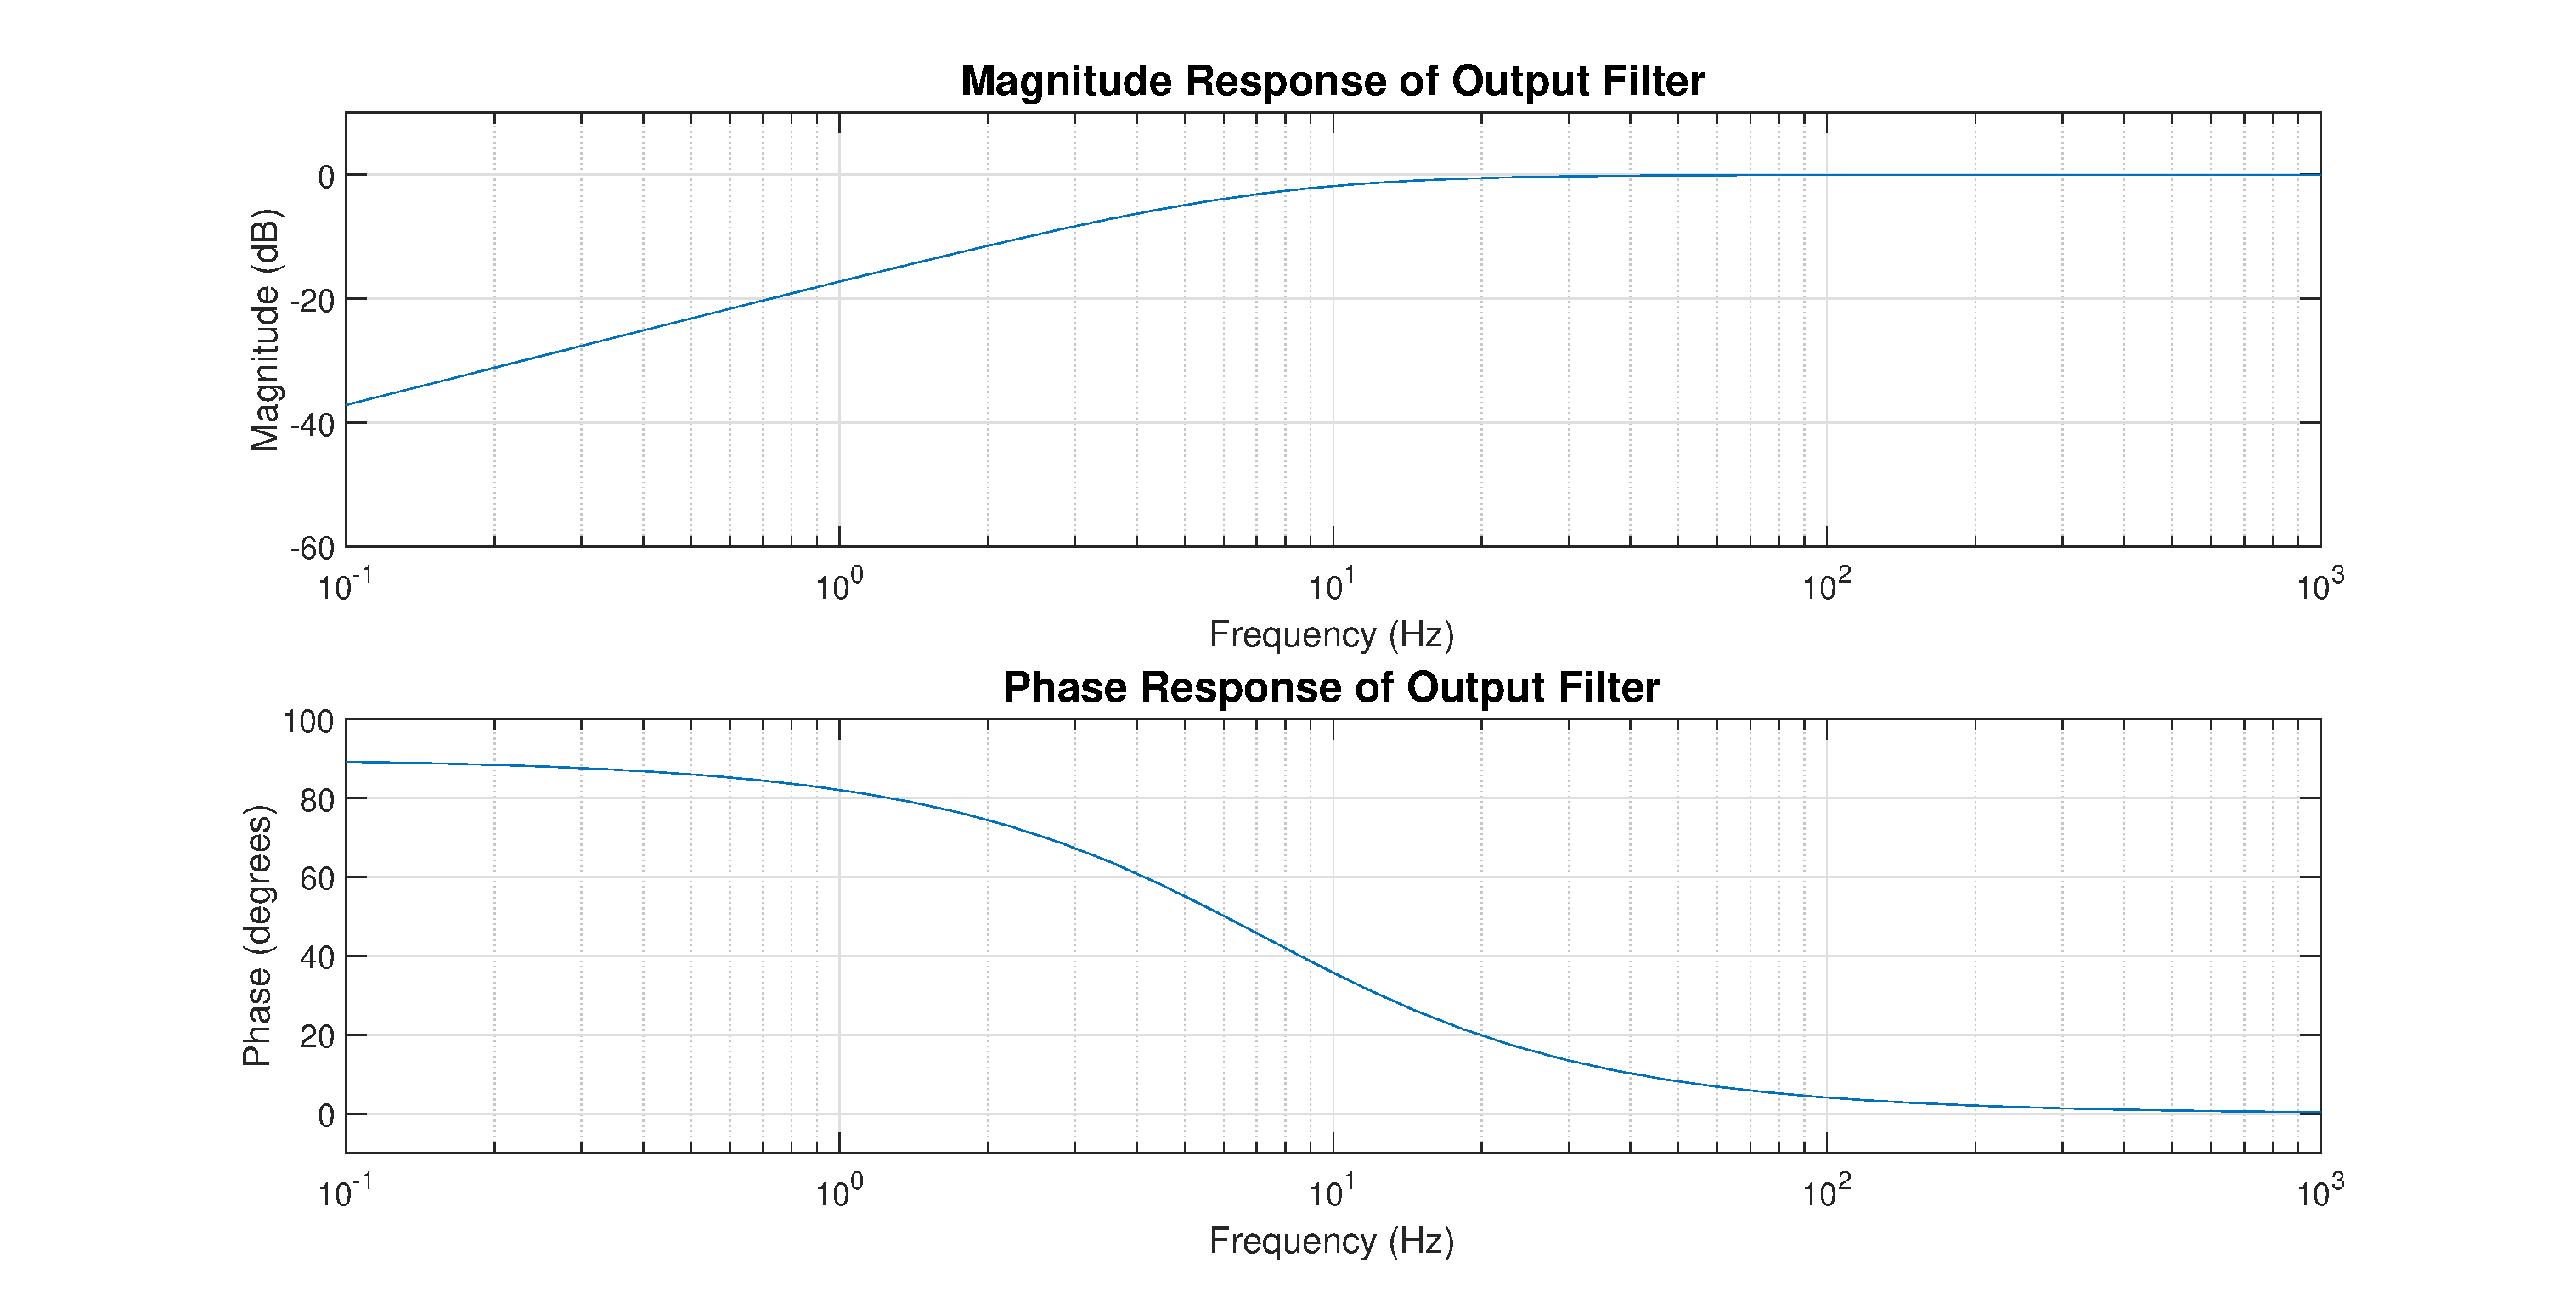
\includegraphics[width=0.5\textwidth]{output_filter.eps}
\caption{Frequency response of high-pass filter at the output of AIC23 audio codec}
\label{fig:output_filter_pranav}
\end{figure}

The analogue filter at the output is designed to block the DC component however, it cannot be implemented perfectly. As calculated above, the cut-off frequency is $7.18Hz$. When a $10Hz$ sine wave with $V_{rms}=1.90V$ is used as an input, the output is not only attenuated but is also skewed. When the frequency of the input wave is reduced to $5Hz$, both effects become more pronounced. The skewing is due to the fact that the analogue filter has a non-linear phase response at these frequencies. Besides skewing, the amplitude of the output wave also decreases with a decrease in frequency. The decay in amplitude is due to the high-pass nature of the filter. These observations are illustrated in Figure \ref{fig:output_filter}.

\begin{figure}[H]
\centering
\includegraphics[width=0.49\textwidth]{ex1_20Hz_output.JPG}
\includegraphics[width=0.49\textwidth]{ex1_10Hz_output.JPG}
\caption{Skewing of output waveform at low frequencies}
\label{fig:output_filter}
\end{figure}

\subsection{Fourier Series of a Rectified Sine Wave}\label{sec:fourier_series_of_a_rectified_sine_wave}

One of the most important learning lessons from laboratory 3 is that simple operations in the time domain have very intricate implications in the frequency domain. Taking the absolute value of a sample seems simple enough in the time domain, however it causes harmonics of the fundamental frequency to appear in the frequency spectrum. This is explained mathematically by considering the Fourier Series of a sinusoid.

The Fourier Series of a signal $f(x)$ is represented as:

\begin{equation}
    f(x) = \frac{1}{2}a_{0} + \sum_{n=1}^{\infty}a_{n}cos(nx) + b_{n}sin(nx)
\end{equation}

The process of calculating the coefficients of the Fourier Series is called Fourier Analysis. The equations below are used for Fourier Analysis:

\begin{align}
    a_{0}   &= \frac{1}{\pi}\int_{-\pi}^{\pi}f(x)dx\label{eq:dc_com}\\ 
    a_{n}   &= \frac{1}{\pi}\int_{-\pi}^{\pi}f(x)cos(nx)dx\label{eq:a_com}\\ 
    b_{n}   &= \frac{1}{\pi}\int_{-\pi}^{\pi}f(x)sin(nx)dx \label{eq:b_com}
\end{align}

To find the DC components of the rectified sine wave, equation (\ref{eq:dc_com}) is used:

\begin{align}
    a_{0}   &= -\frac{1}{\pi}\int_{-\pi}^{0}sin(x)dx + \frac{1}{\pi}\int_{0}^{\pi}sin(x)dx\\
            &= \frac{2}{\pi}\int_{0}^{\pi}sin(x)dx\\
            &= \frac{2}{\pi}\left[-cos(x)\right]_{0}^{\pi}\\
            &= \frac{4}{\pi}
\end{align}

Next, to find the general form of the $a_{n}$ components, equation (\ref{eq:a_com}) is used:

\begin{align}
    a_{n}   &= -\frac{1}{\pi}\int_{-\pi}^{0}sin(x)cos(nx)dx + \frac{1}{\pi}\int_{0}^{\pi}sin(x)cos(nx)dx\\
            &= \frac{2}{\pi}\int_{0}^{\pi}sin(x)cos(nx)dx\\
            &= \frac{1}{\pi}\int_{0}^{\pi}sin(x+nx)+sin(x-nx)dx\\
            &= \frac{1}{\pi}\left[-\frac{cos(x+nx)}{1+n}-\frac{cos(x-nx)}{1-n}\right]_{0}^{\pi}\\
            &= \frac{1}{\pi}\left[\frac{cos(x+nx)}{1+n}+\frac{cos(x-nx)}{1-n}\right]_{\pi}^{0}\\
            &= \frac{1}{\pi}\Bigg(\left(\frac{1}{1+n}+\frac{1}{1-n}\right) - \left(\frac{cos(\pi+n\pi)}{1+n}+\frac{cos(\pi-n\pi)}{1-n}\right)\Bigg)\\
            &= \frac{1}{\pi}\Bigg(\frac{2}{1-n^{2}}-\frac{cos(\pi)cos(n\pi)-sin(\pi)sin(n\pi)}{1+n}-\frac{cos(\pi)cos(n\pi)+sin(\pi)sin(n\pi)}{1-n}\Bigg)\\
            &= \frac{1}{\pi}\Bigg(\frac{2}{1-n^{2}}+\frac{cos(n\pi)}{1+n}+\frac{cos(n\pi)}{1-n}\Bigg)\\
            &= \frac{1}{\pi}\left(\frac{2}{1-n^{2}}+\frac{2}{1-n^{2}}cos(n\pi)\right)\\
            &= -\frac{2}{\pi} \ \frac{1+cos(n\pi)}{n^{2}-1}
\end{align}

Lastly, to find the general form of the $b_{n}$ components, equation (\ref{eq:b_com}) is used:

\begin{align}
    b_{n}   &= -\frac{1}{\pi}\int_{-\pi}^{0}sin(x)sin(nx)dx + \frac{1}{\pi}\int_{0}^{\pi}sin(x)sin(nx)dx\\
            &= \frac{2}{\pi}\int_{0}^{\pi}sin(x)sin(nx)dx\\
            &= \frac{1}{\pi}\int_{0}^{\pi}cos(x-nx)-cos(x+nx)dx\\
            &= \frac{1}{\pi}\left[\frac{sin(x-nx)}{1-n}-\frac{sin(x+nx)}{1+n}\right]_{0}^{\pi}\\
            &= \frac{1}{\pi}\Bigg(\left(\frac{sin(\pi-n\pi)}{1-n}-\frac{sin(\pi+n\pi)}{1+n}\right)+\left(0\right)\Bigg)\\
            &= \frac{1}{\pi}\Bigg(\frac{sin(\pi)cos(n\pi)-cos(\pi)sin(n\pi)}{1-n}-\frac{sin(\pi)cos(n\pi)+cos(\pi)sin(n\pi)}{1+n}\Bigg)\\
            &= \frac{1}{\pi}\Bigg(\frac{sin(n\pi)}{1-n}-\frac{sin(n\pi)}{1+n}\Bigg)\\
            &= \frac{1}{\pi} \ \frac{2n}{1-n^{2}} \ sin(n\pi)
\end{align}

From the Fourier Analysis applied above, it is clear that the rectified sine wave has the following equation:

\begin{equation}\label{eq:rectified_sine_wave}
    f(x)=|sin(x)|=\frac{2}{\pi}-\frac{4}{\pi}\sum_{n=2,4,6,\cdots}^{\infty}\frac{cos(nx)}{n^2-1}
\end{equation}

As mentioned above, the repercussions of a simple time-domain operation of taking the absolute value has the profound effect of producing an infinitely long Fourier Series. \textbf{It should be noted that a perfect fully-rectified sine wave will only be produced if the output is a sum of infinite harmonics, weighted according to equation (\ref{eq:rectified_sine_wave}).} There are 2 reasons why this is not possible.

\begin{enumerate}
    \item Producing infinite harmonics is not physically possible.
    \item An anti-aliasing filter\footnote{The anti-aliasing filter is a digital filter. The AIC23 audio codec allows for multiple sampling frequencies and thus it only makes sense to have 1 analogue anti-aliasing filter with a cut-off frequency of $48kHz$ to support the maximum sampling frequency of $96kHz$. Anti-aliasing filters for other sampling frequencies are implemented digitally} is placed at the output such that frequencies above $4kHz$ are attenuated.
\end{enumerate}

To compare the quality of the outputs, a $200Hz$ fully-rectified sine wave is graphed next to a $1kHz$ fully rectified sine wave in Figure \ref{fig:compare_output_quality_pranav}. 

\begin{figure}[H]
    \centering
    \includegraphics[width=0.49\textwidth]{ex1_200Hz_output_2.JPG}
    \includegraphics[width=0.49\textwidth]{ex1_1000Hz_output.JPG}
    \caption{Comparison of quality of outputs}
    \label{fig:compare_output_quality_pranav}
\end{figure}

It is clear that the $200Hz$ output has much sharper edges than the $1kHz$ output. The discrepancy in the quality of the outputs is explained by considering the Fourier Series representation the outputs.\\

For the $200Hz$ output:

\begin{equation}
    f_{1}(x) = |sin(2\pi (100)nt)| = \frac{2}{\pi}-\frac{4}{\pi}\Bigg(\frac{cos(2\pi (200)t)}{3}+\frac{cos(2\pi (400)t)}{15} + \frac{cos(2\pi (600)t)}{35} + \cdots\Bigg)
\end{equation}

Whereas for the $1kHz$ output:

\begin{equation}
    f_{2}(x) = |sin(2\pi (500)nt)| = \frac{2}{\pi}-\frac{4}{\pi}\Bigg(\frac{cos(2\pi (1000)t)}{3}+\frac{cos(2\pi (2000)t)}{15} + \frac{cos(2\pi (3000)t)}{35} + \cdots\Bigg)
\end{equation}

The theoretical spectrum of the two output waves are plotted in Figure \ref{fig:theoretical_spectrum}. These were generated using a MATLAB script which is presented in Appendix B. Note that the spectra are plotted up to $16kHz$ however the low-pass anti-aliasing filter will attenuate frequencies above $4kHz$. 

\begin{figure}[H]
    \centering
    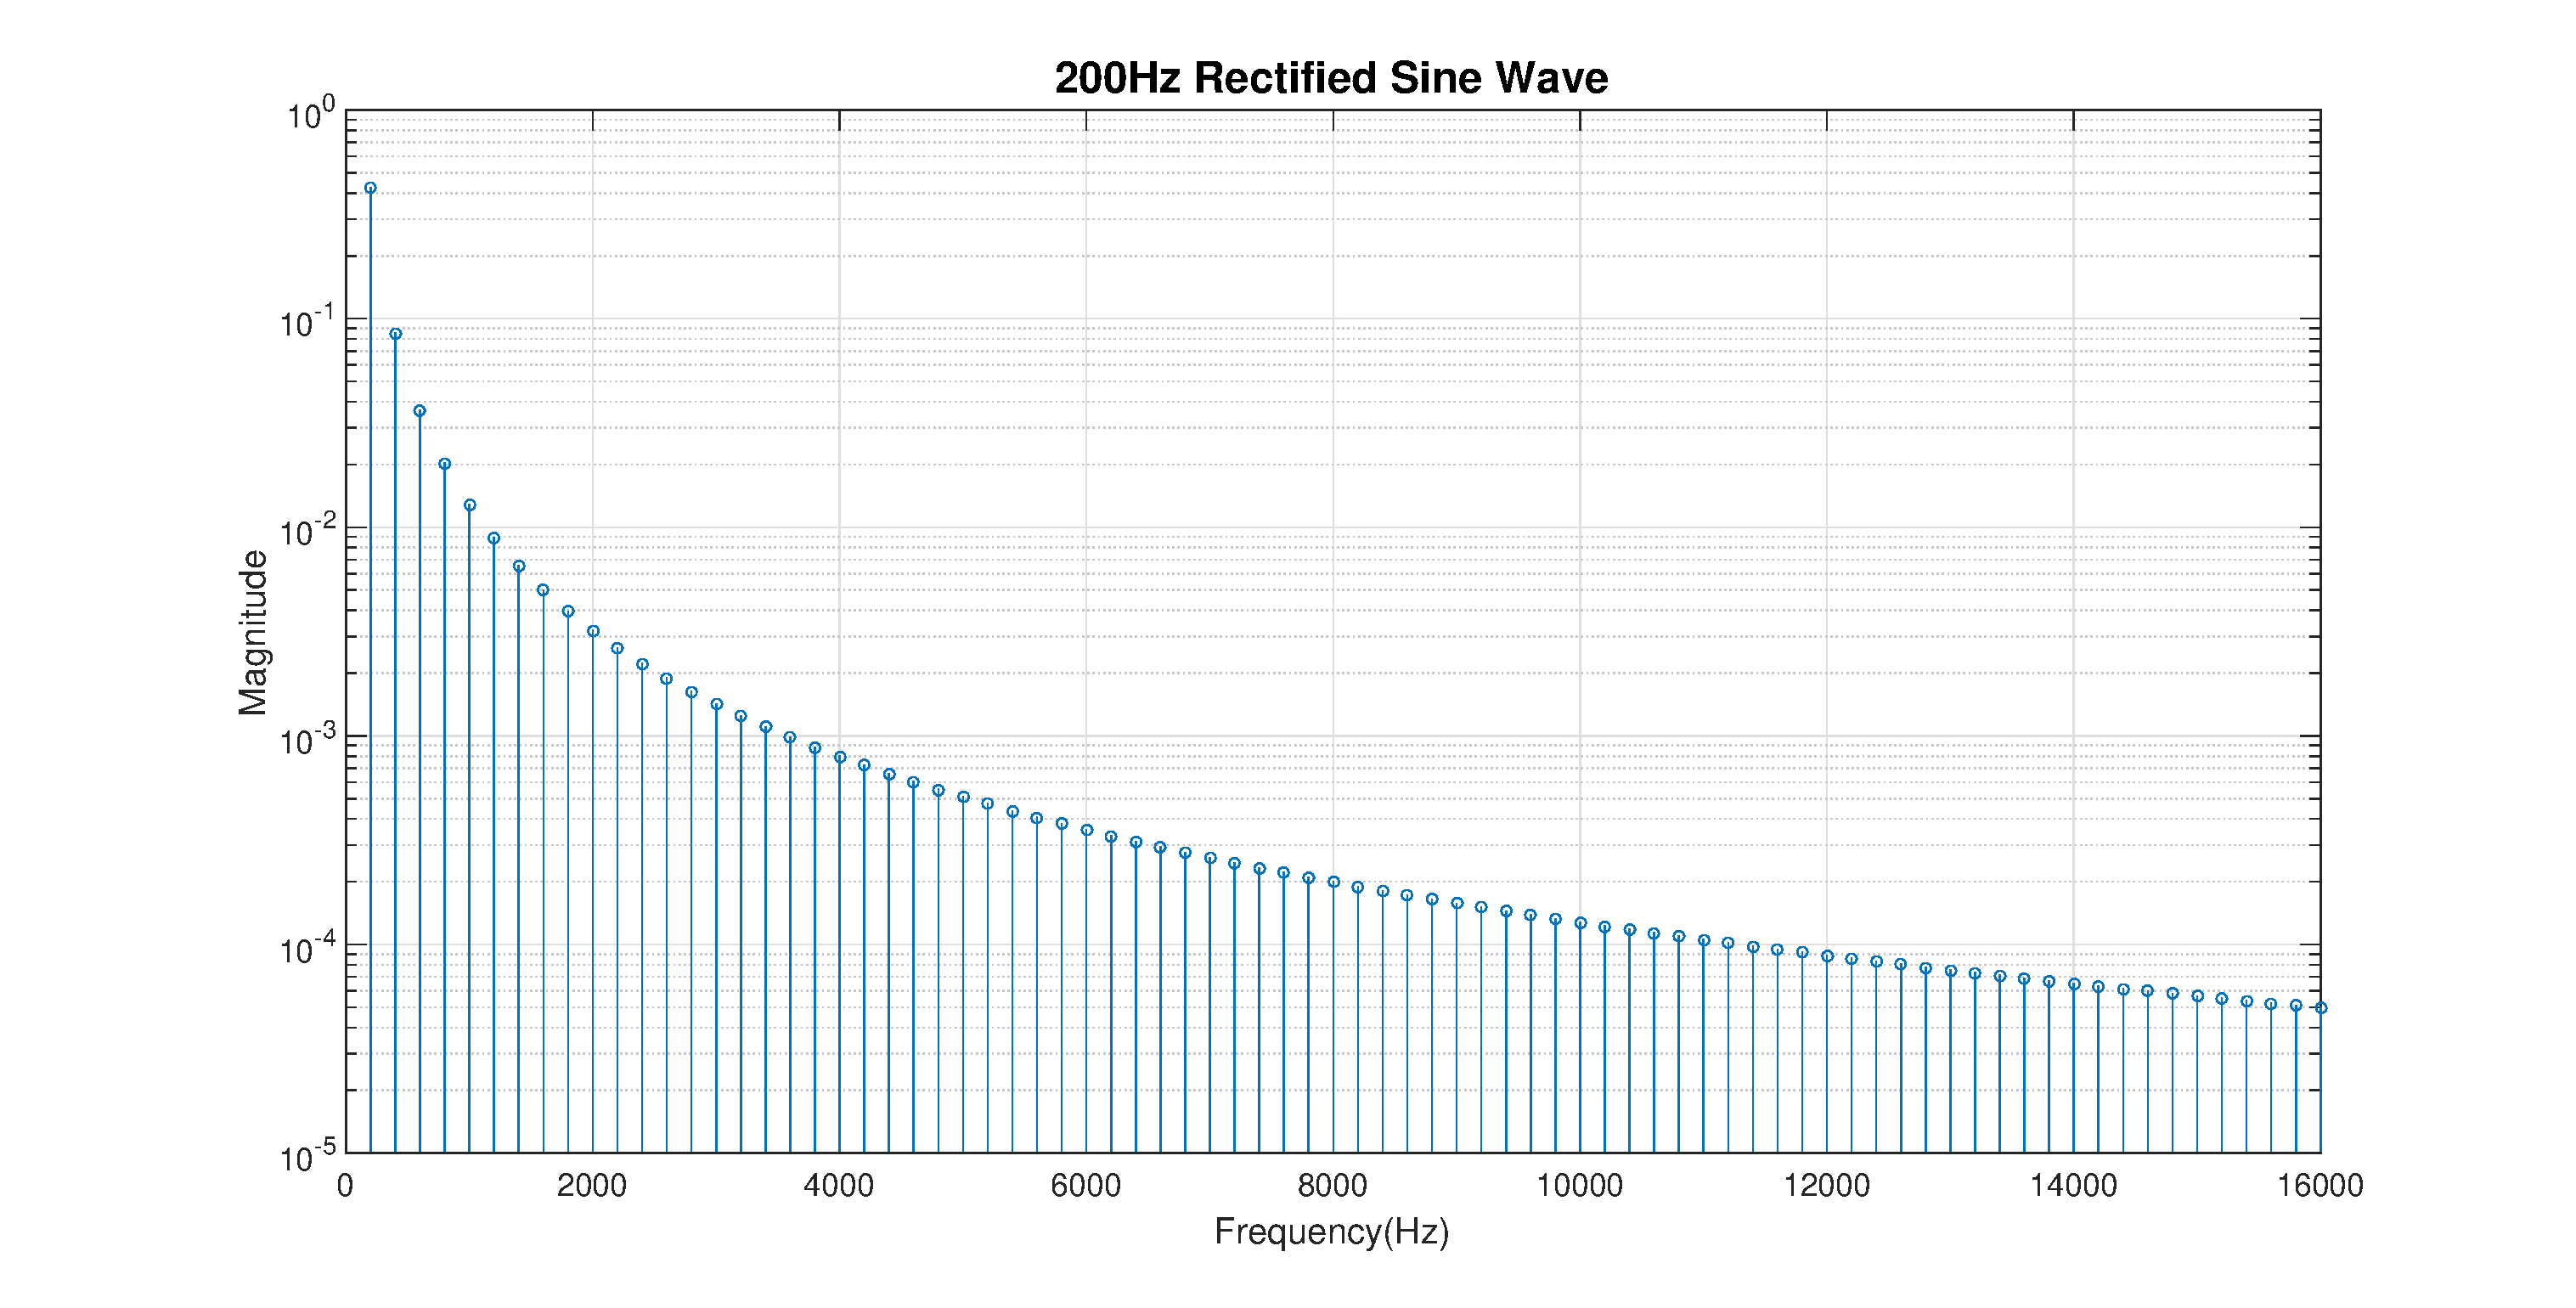
\includegraphics[width=0.49\textwidth]{200Hz_rectified_sine_wave.eps}
    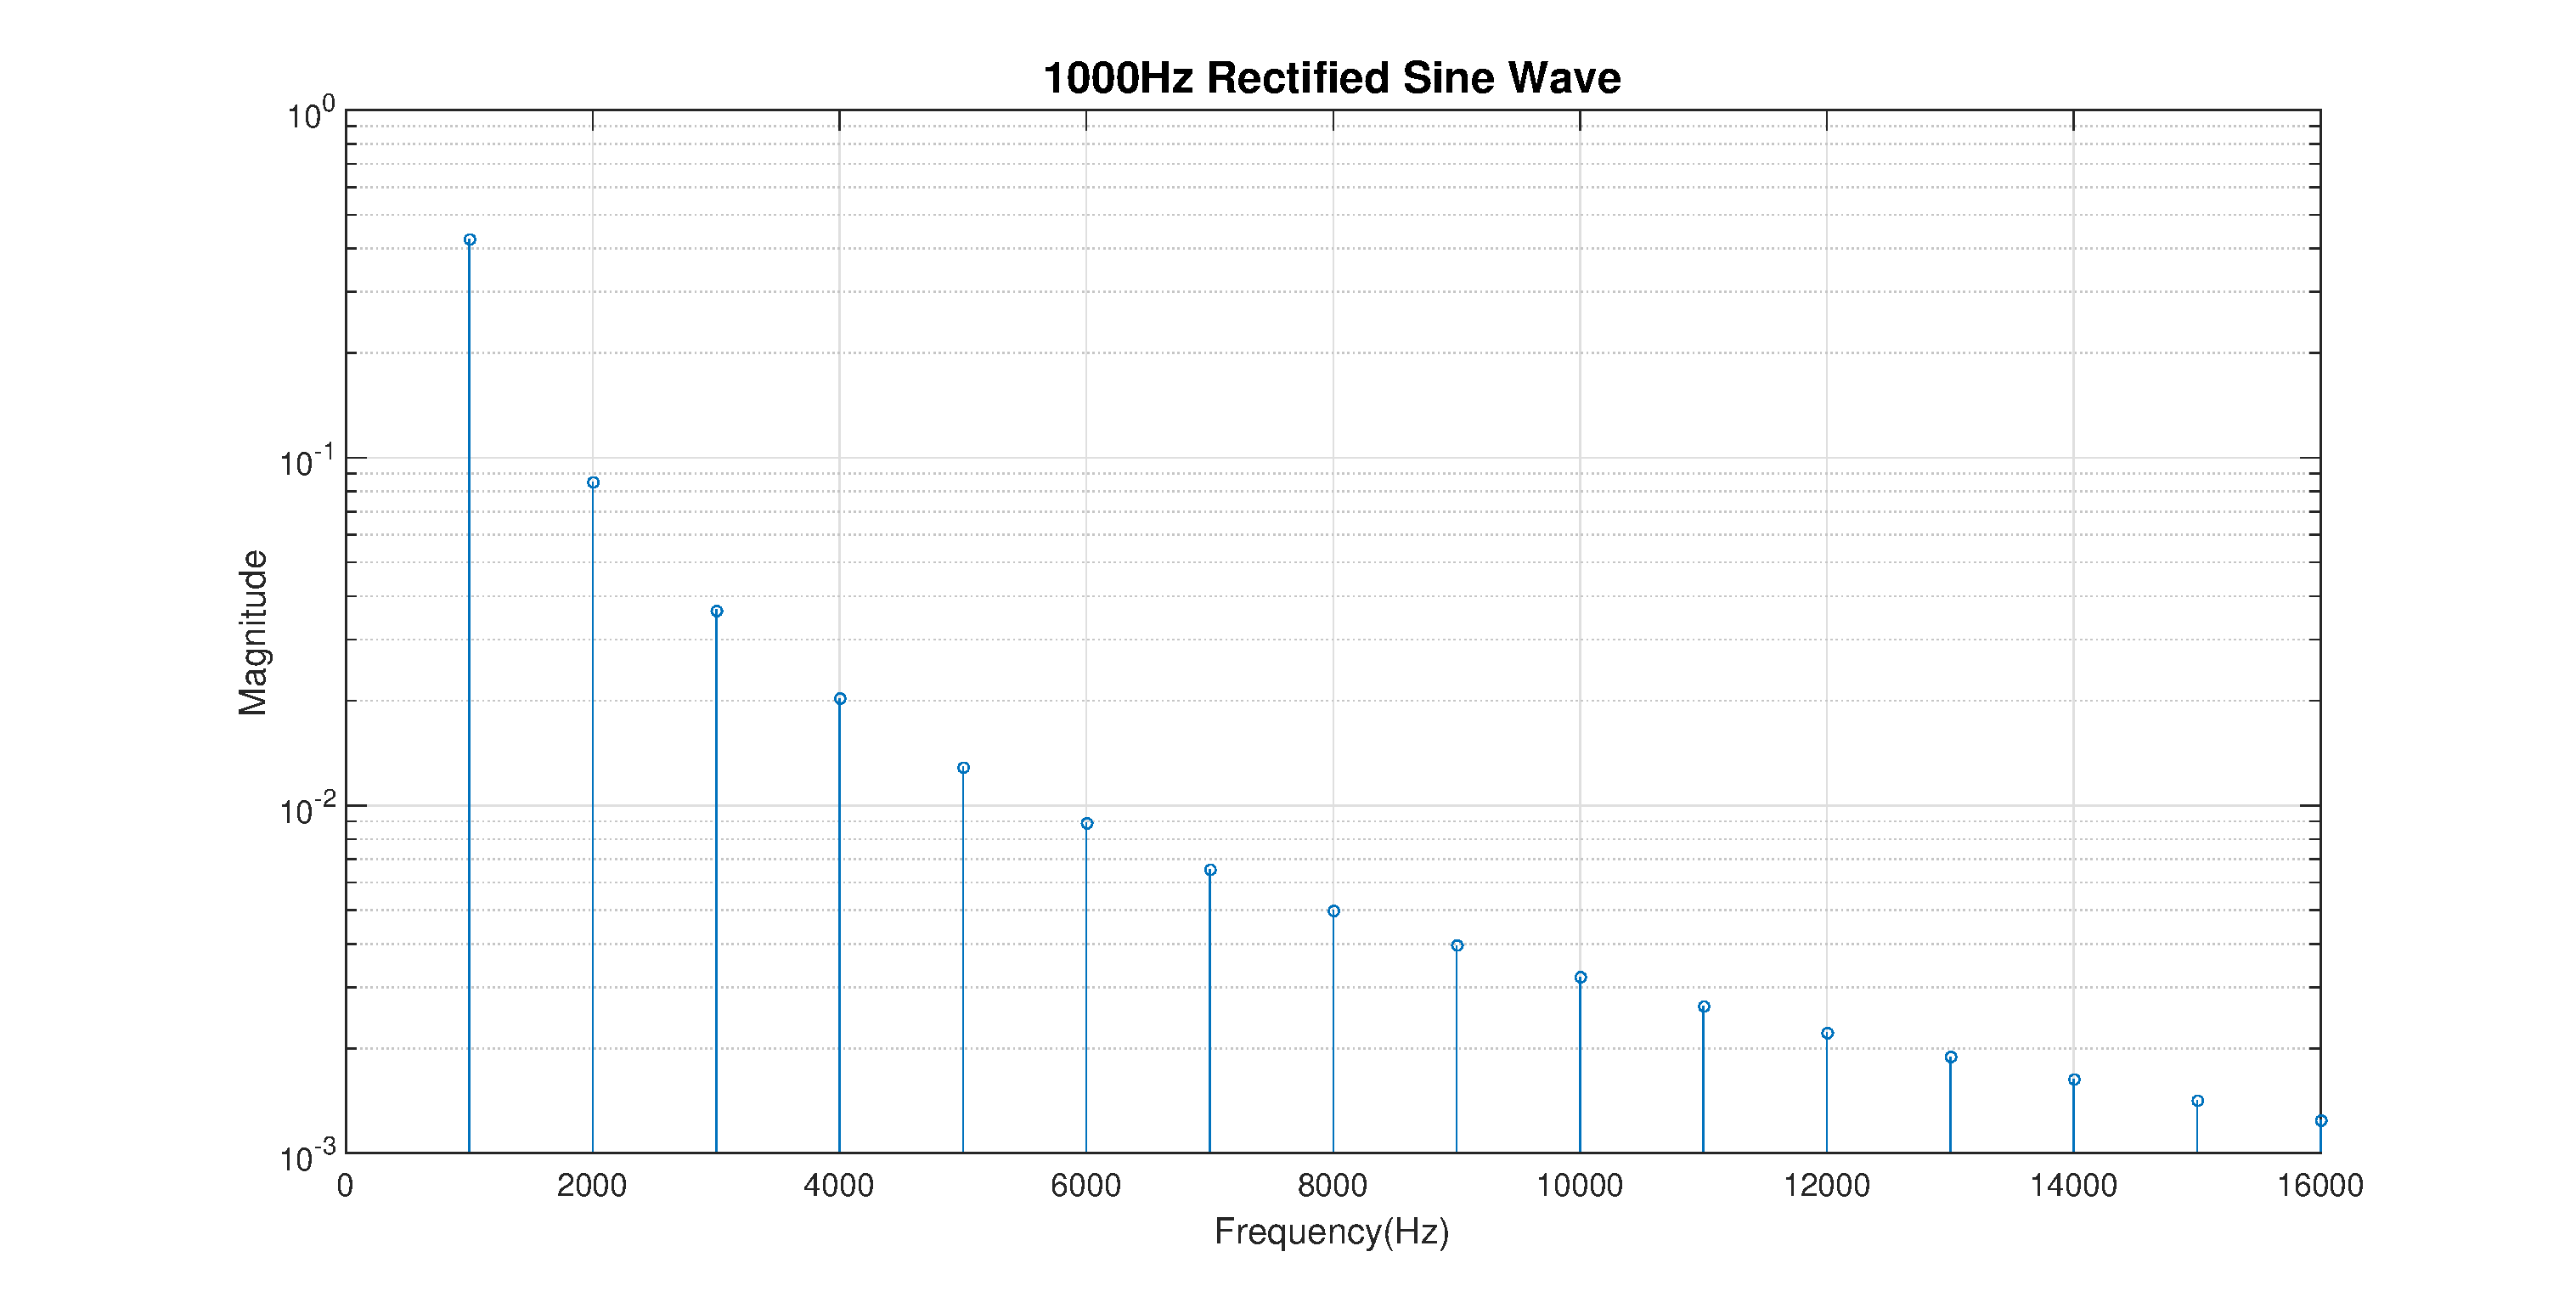
\includegraphics[width=0.49\textwidth]{1000Hz_rectified_sine_wave.eps}
    \caption{Theoretical spectrum}
    \label{fig:theoretical_spectrum}
\end{figure}

From Figure \ref{fig:theoretical_spectrum} it is clear that before the $4kHz$ cut-off frequency is reached, $f_{1}(x)$ will have 20 terms in its Fourier Series whereas $f_{2}(x)$ will only have 4 terms. The shorter Fourier Series accounts for imperfections in the output, most notably the rounded edges.\\

The findings are corroborated by the Fast Fourier Transform (FFT) plots in Figure \ref{fig:compare_output_fft_pranav}.

\begin{figure}[H]
    \centering
    \includegraphics[width=0.49\textwidth]{ex1_200Hz_output_2_FFT.JPG}
    \includegraphics[width=0.49\textwidth]{ex1_1000Hz_output_FFT.JPG}
    \caption{FFT of $200Hz$ and $1kHz$ output waves}
    \label{fig:compare_output_fft_pranav}
\end{figure}

The truncation of the Fourier Series also has a profound effect at high frequencies. The Fourier Series of a $3kHz$ output has the following form:

\begin{equation}\label{eq:3000Hz_output_FS}
    f_{3}(x) = |sin(2\pi (1500)nt)| = \frac{2}{\pi}-\frac{4}{\pi}\Bigg(\frac{cos(2\pi (3000)t)}{3}+\frac{cos(2\pi (6000)t)}{15} + \frac{cos(2\pi (9000)t)}{35} + \cdots\Bigg)
\end{equation}
\newpage
Equation (\ref{eq:3000Hz_output_FS}) maps to the frequency spectrum shown in Figure \ref{fig:3000Hz_spectrum}:

\begin{figure}[H]
    \centering
    \includegraphics[width=0.7\textwidth]{3000Hz_rectified_sine_wave.eps}
    \caption{Frequency spectrum of $3kHz$ rectified wave}
    \label{fig:3000Hz_spectrum}
\end{figure}

A serve shortening of the Fourier Series is expected when a $1.5kHz$ sine wave is used as an input. There is only one spectral component below $4kHz$ and thus the output should be a $3kHz$ sine wave that is not rectified. Figure \ref{fig:3000Hz_output} shows the findings. A severely distorted output was observed and thus the FFT of the output is also provided in Figure \ref{fig:3000Hz_output}.

\begin{figure}[H]
    \centering
    \includegraphics[width=0.49\textwidth]{ex1_3000Hz_output}
    \includegraphics[width=0.49\textwidth]{ex1_3000Hz_output_FFT}
    \caption{$1.5kHz$ input produces an output that is not rectified}
    \label{fig:3000Hz_output}
\end{figure}

A very strong spectral component at $3kHz$ is observed. This is expected. However, spectral components at other frequencies also exist. Their existence is explained in the next section.

\newpage
\subsection{Frequency Domain Analysis}

As alluded to in the previous section, two interesting phenomena were observed when a $1.5kHz$ sine wave is used as an input; firstly the signal's amplitude is modulated and secondly, the signal's FFT had multiple harmonics that equation (\ref{eq:rectified_sine_wave}) does not account for. The phenomena is more pronounced when a $1.9kHz$ sine wave is used as an input. 

\begin{figure}[H]
    \centering
    \includegraphics[width=0.49\textwidth]{ex1_3800Hz_output_cursor}
    \includegraphics[width=0.49\textwidth]{ex1_3800Hz_output_FFT}
    \caption{Aliasing and amplitude modulation with $1.9kHz$ sine wave used as an input}
\end{figure}


Explanation of this requires mathematical analysis in the frequency domain instead of in the time domain. There are three important concepts that are needed to understand this interesting phenomena.

\begin{enumerate}
    \item \textbf{Taking the absolute value of a sampled sine wave is equivalent to sampling a fully-rectified wave of double the frequency and doing no processing. In memory, both values result in the same floating point number. Thus, for the following analysis, it is assumed that a rectified sine wave is provided as an input.}
    \item \textbf{Equation (\ref{eq:rectified_sine_wave}) shows that the frequency spectrum of a fully-rectified sine wave is not band-limited\footnote{Albeit the equation shows the Fourier Series and not the spectral components, the coefficients of the Fourier Series are directly mapped into the frequency domain, and thus this loose use of language is acceptable.}. This means that no matter what sampling frequency is used, aliasing will still be present. Aliasing, however was not observed up until this point because the high frequency spectral components decay and the aliased harmonics were insignificant}  
    \item \textbf{The anti-aliasing filter is not an ideal brick wall filter\footnote{An ideal filter will require implementing a filter with an infinite number of coefficients.} and thus, spectral components above $4kHz$ may appear in the output.}
\end{enumerate}


The spectrum of a $3.8kHz$ fully-rectified sine wave is shown in Figure \ref{fig:fully_rectified_sine_wave_spectrum}. As mentioned above this, it is assumed that a $3.8kHz$ fully-rectified sine wave is used as the input. 

\begin{figure}[H]
    \centering
    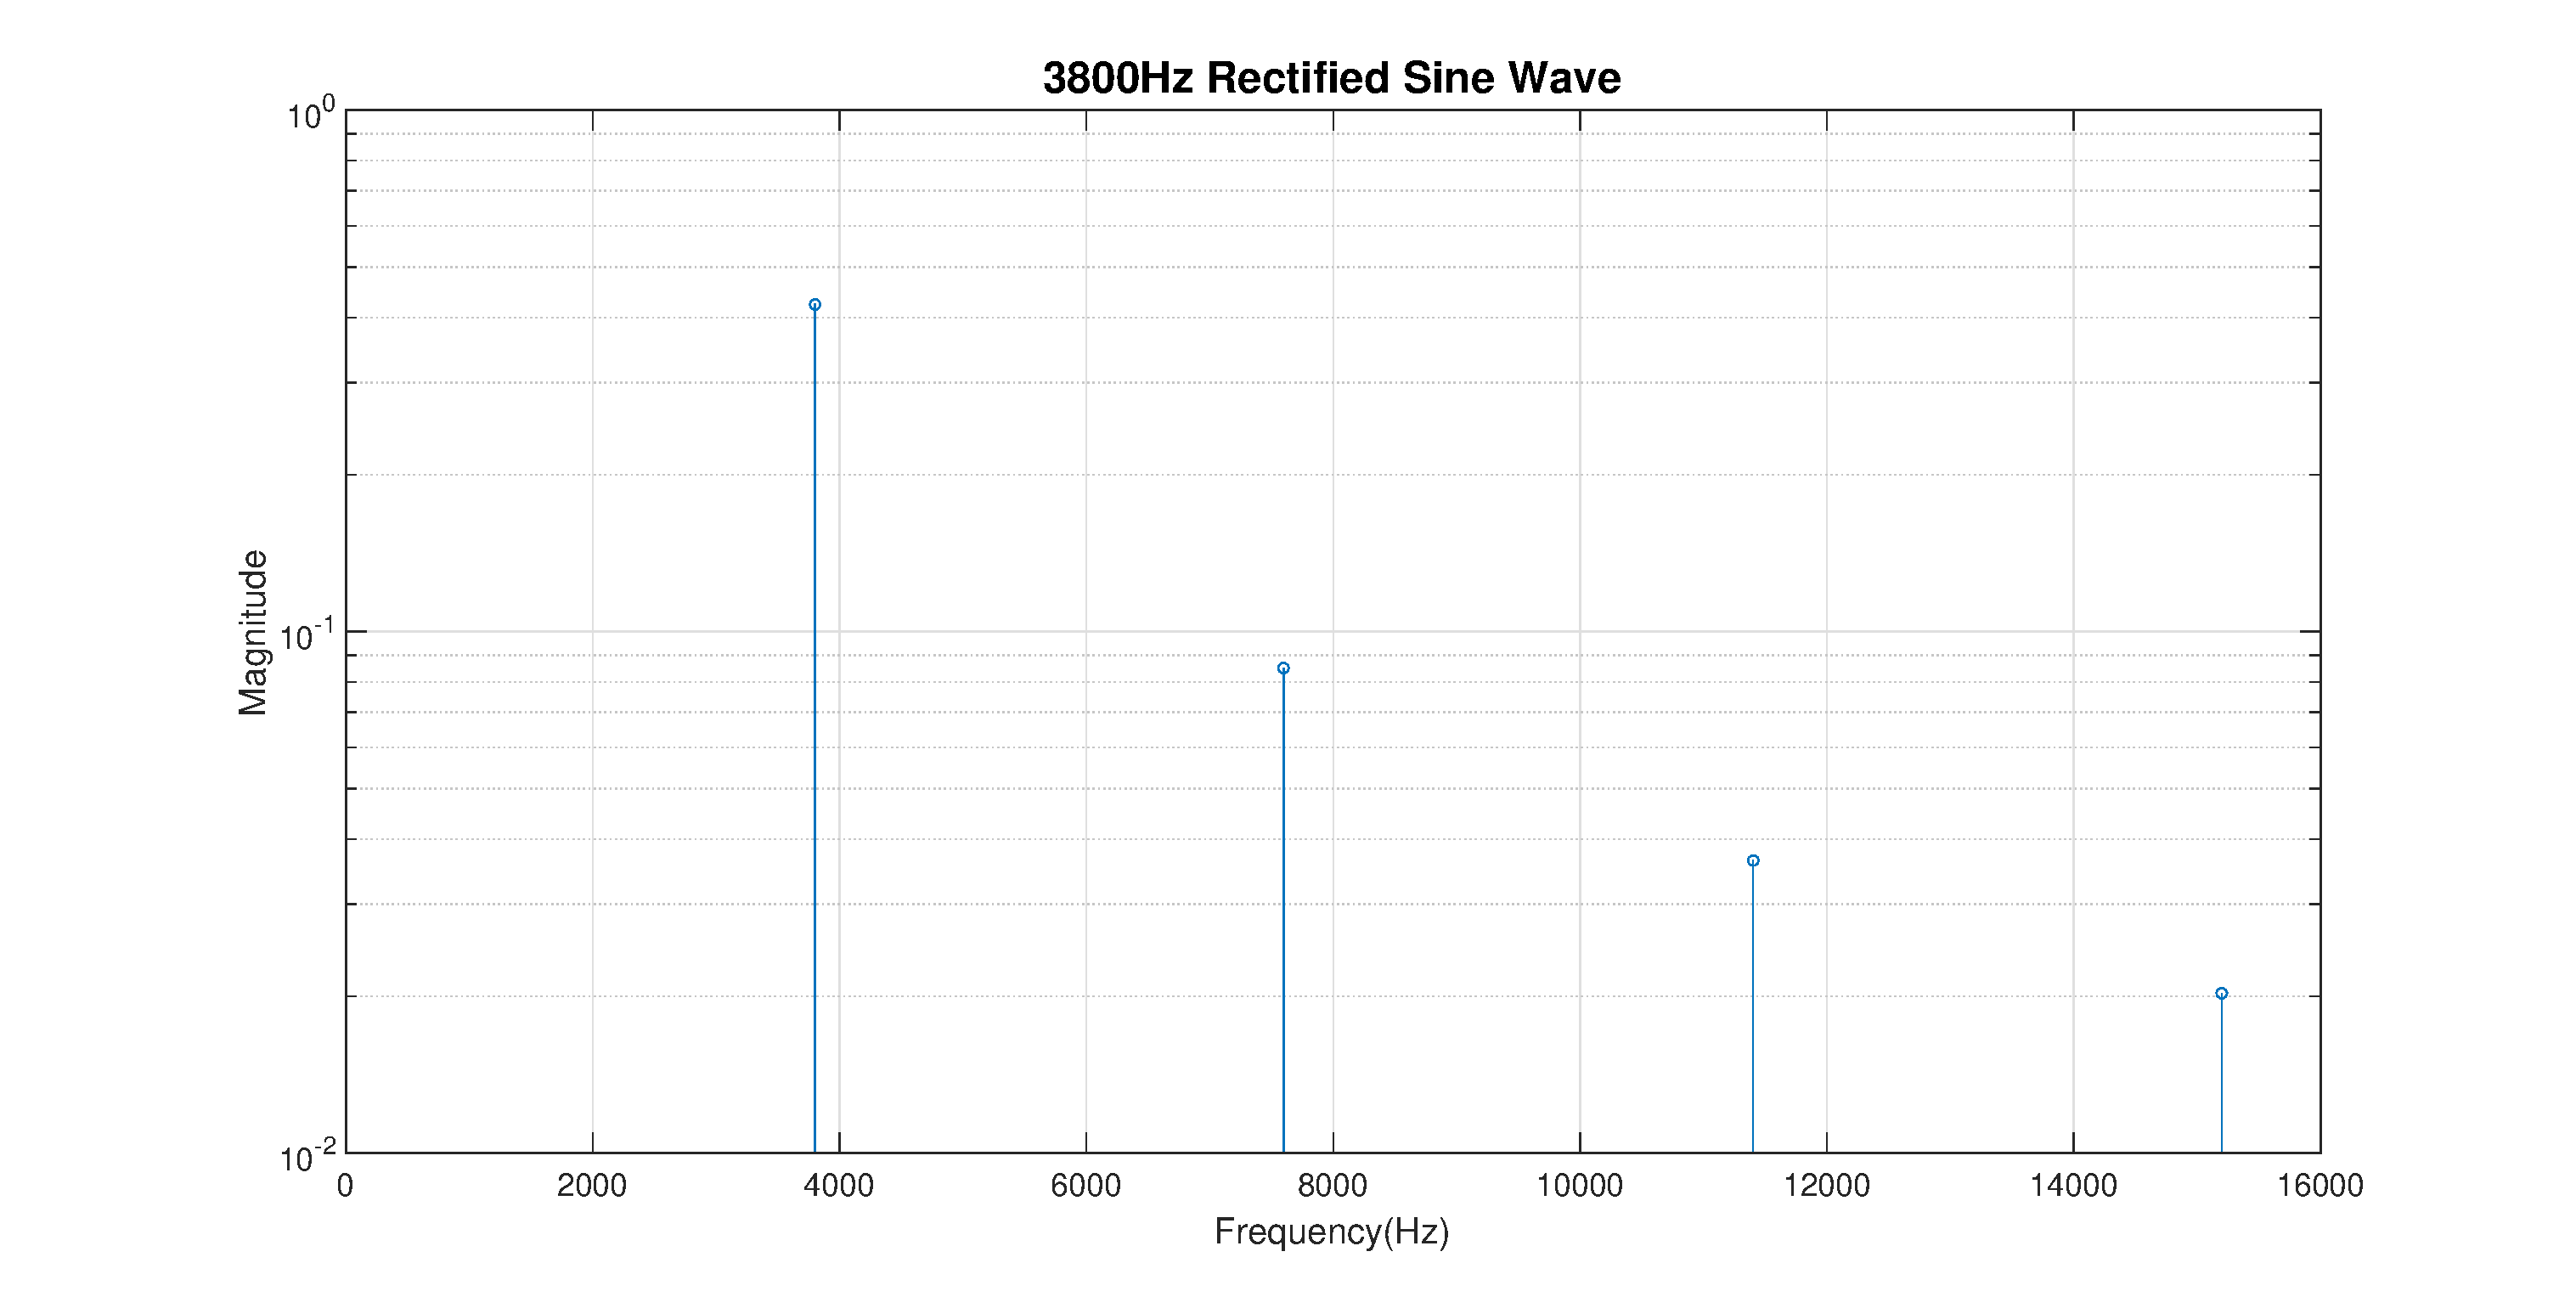
\includegraphics[width=0.6\textwidth]{3800Hz_rectified_sine_wave_not_sampled}
    \caption{Frequency spectrum of a $3.8kHz$ rectified sine wave}
    \label{fig:fully_rectified_sine_wave_spectrum}
\end{figure}

The spectrum of a fully-rectified sine wave that has been sampled at $8kHz$ is shown is Figure \ref{fig:fully_rectified_sine_wave_spectrum_sampled}.

\begin{figure}[H]
    \centering
    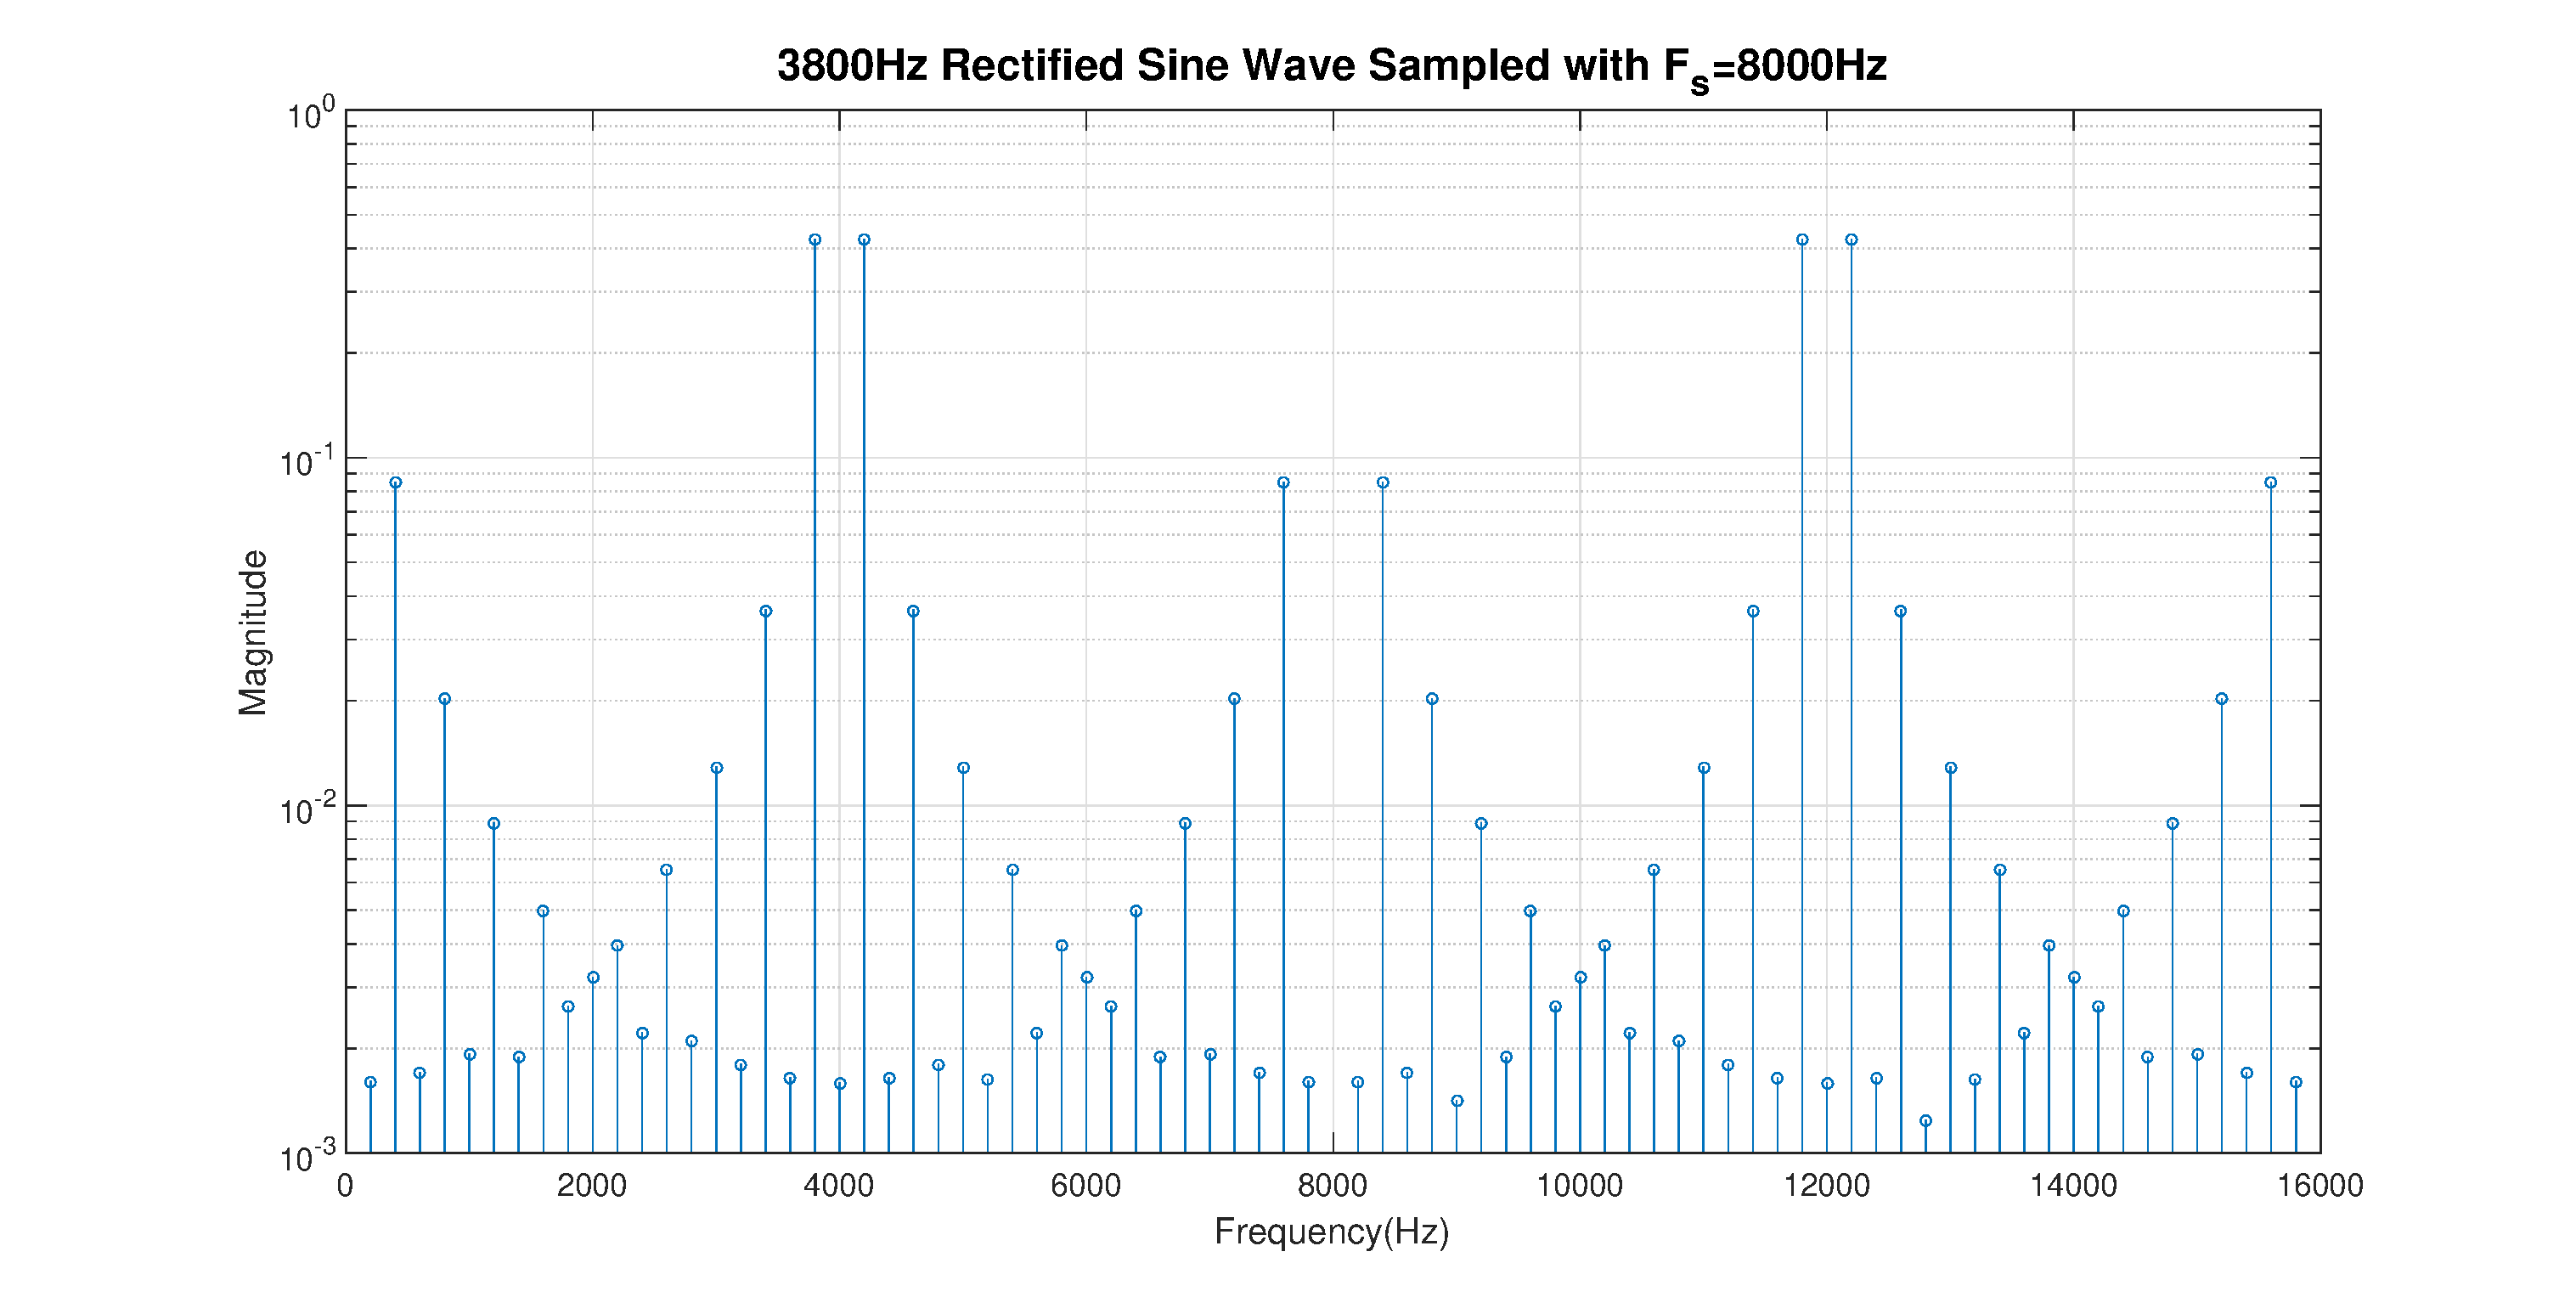
\includegraphics[width=0.6\textwidth]{3800Hz_rectified_sine_wave}
    \caption{Frequency spectrum of a $3.8kHz$ rectified sine wave sampled at $8kHz$}
    \label{fig:fully_rectified_sine_wave_spectrum_sampled}
\end{figure}


Thus, it is clear that the sampling process has caused aliasing to occur. In this case, the aliasing is observable because spectral components above $4kHz$ are significant. The aliasing explains the multiple harmonics that are observed in the FFT of the output. It alone cannot explain the amplitude modulation. \textbf{The amplitude modulation occurs because the anti-aliasing filter is not perfect. The anti-aliasing filter does not fully attenuate a harmonic at $4.2kHz$. This together with the fundamental harmonic at $3.8kHz$ cause amplitude modulation that is observed.} Equation (\ref{eq:trig_identity}) shows what happens when two sine waves of different frequencies are added together. 

\begin{align}
    acos(\theta) + bcos(\phi)   &= (a-b)cos(\theta) + bcos(\theta) + bcos(\phi)\\
                                &= (a-b)cos(\theta) + bcos(\frac{\theta + \phi}{2})cos(\frac{\theta-\phi}{2})\label{eq:trig_identity}
\end{align}

Applying the above trigonometric identity, equation (\ref{eq:amplitude_modulation}) explains the $200Hz$ envelope that is observed. \textbf{It should be noted that although a $200Hz$ envelope is observed in the time domain, this component will not appear in frequency domain. The time domain view only shows the effect that is manifested as a result of equation (\ref{eq:amplitude_modulation}).}

\begin{align}
    sin(2\pi (3800)t)+sin(2\pi (4200)t) &= 2sin(2\pi \frac{(3800+4200)}{2}t)cos(2\pi \frac{(3800-4200)}{2}t)\\
                                        &= 2sin(2\pi (4000)t)cos(2\pi (200)t)\label{eq:amplitude_modulation}
\end{align}

\subsection{Effective Folding Frequency}

Lastly, because of a fully-rectified sine wave has twice the frequency as that of a sine wave, the effective folding frequency due to sampling at $8kHz$ is at $2kHz$ and not at $4kHz$. Thus, using a $3.8kHz$ sine wave as an input should result in the same output as using a $200Hz$ sine wave. This is confirmed in Figure \ref{fig:3800Hz_input}.

\begin{figure}[H]
    \centering
    \includegraphics[width=0.49\textwidth]{ex1_3800Hz_input}
    \includegraphics[width=0.49\textwidth]{ex1_3800Hz_input_FFT}
    \caption{Output when $3.8kHz$ sine wave is used as input}
    \label{fig:3800Hz_input}
\end{figure}

\subsection{Further Discussion}
It is important to note that the phenomena observed above can be viewed from another perspective. To explain how multiple unexpected harmonics appear in the frequency spectrum of the fully-rectified sine wave, the convolution between the spectrum of a sine wave and a square wave can be considered. \textbf{The process of taking an absolute value was viewed above as simply sampling a fully-rectified wave. It can however also be viewed as the multiplication of a sine wave and a square wave in the time-domain. The mathematical analysis requires computing the convolution of two spectra and can be performed easily on MATLAB.} It provides the same results but the discussion above is more intuitive. \\

It can be concluded that to obtain a proper fully-rectified sine wave without,
\begin{itemize}
    \item Significant rounding of the edges
    \item Aliasing
    \item Amplitude modulation
    \item Amplitude attenuation
    \item Skewing
\end{itemize}
The frequencies have to be limited to $10Hz$ to $400Hz$.

\newpage
\section{Exercise 2}

In exercise 2, the sine wave is generated using a look-up table instead of taking as input a sine wave generated by software or hardware. An ISR is run when the McBSP is ready to write a sample rather than when it has received one.

\subsection{Interrupt Initialisation}
The configuration file was modified to account for this change\footnote{The interrupt source was changed from {\tt MCSP\_1\_Receive} to {\tt MCSP\_1\_Transmit}. The function {\tt init\_HWI} was also modified to map the ISR to the correct physical event {\tt IRQ\_EVT\_XINT1}}.\\

\begin{lstlisting}[language=C, frame = single, caption=Interrupt initialisation for exercise 2]
void init_HWI(void)
{
	IRQ_globalDisable();            // Globally disables interrupts
	IRQ_nmiEnable();                // Enables the NMI interrupt (used by the debugger)
	IRQ_map(IRQ_EVT_XINT1,4);       // Maps an event to a physical interrupt
	IRQ_enable(IRQ_EVT_XINT1);      // Enables the event
	IRQ_globalEnable();             // Globally enables interrupts
} 
\end{lstlisting}

\subsection{Full Wave Rectification Function}
Listing \ref{lst:c-code} shows the two functions necessary to implement a full wave rectification using a look up table. Firstly, the function {\tt sine\_init} initialises a look-up table that contains 256 samples from 1 cycle of a sine wave. A more involved discussion of this generation process was presented in the previous report and is thus excluded from this report. Next, the function {\tt ISR\_AIC} defines the ISR. Note that the increment value is re-calculated each time the ISR is called to enable the use of the watch window to change the signal frequency. The number of samples that are skipped is stored in the variable {\tt increment} which can be monitored in the watch window for debugging purposes\footnote{Again, a more involved discussion is provided in the previous report.}.\\

\begin{lstlisting}[language=C, frame = single, caption=Code to generate interrupt driven rectified sine wave (using a look-up table), label = lst:c-code]
void sine_init(void){
    // initilisies look-up table
    // RESOLUTION provides the option to only store one quadrant of the sine wave
    
    int i;
    // Store an entire sine wave (or single quadrant) in look-up table
    for(i=0; i<SINE_TABLE_SIZE; i++)
        table[i] =  sin(2*PI*i/(RESOLUTION*SINE_TABLE_SIZE));
}

void ISR_AIC(void){
    // interrupt service routine to fully rectify sine wave
    // uses global variables, increment, index, table
    // code allows use of watch window to monitor variables
    // RES_OPTIMISE allows use of optimised code
    
    // calculate increment here so that we can exploit watch window
    increment = sine_freq*SINE_TABLE_SIZE*RESOLUTION/sampling_freq;
    
    index+=increment;
    
    // modulo index so that we do not exceed size of look-up table	   
    index = fmod(index,SINE_TABLE_SIZE*RESOLUTION);
    
    // Read sample then write absolute value
    // Note: to create a visible scope output, we magnify by 30000
    #ifdef RES_OPTIMISE
        mono_write_16Bit(abs( 30000*getSineValue(round(index)) ));
    #else
        mono_write_16Bit(abs( 30000*table[(int)round(index)] ));
    #endif
}


\end{lstlisting}

Since the ISR should be as fast as possible, an option to disable resolution optimisation, using an {\tt \#ifdef} directive defined in the pre-processor statements, is included. If resolution optimisation is enabled, only one quadrant of the sine wave is stored and the function {\tt getSineValue} is called to manipulate the index so as to output the correct value from the look-up table. \\

\begin{lstlisting}[language=C, frame=single, caption=Optimised code]
/********************************** getSineValue() **********************************/
// This function is used if resolution optimisation is enabled
// Since only one quadrant of the sine wave is stored
// this function returns the correct entry in the look-up table
// index1 used to prevent confusion with global variable index
// index1 is within function's local scope
#ifdef RES_OPTIMISE
	float getSineValue(int index1){
	    int quadrant = index1/SINE_TABLE_SIZE; // Quadrant number
	    int modulo = index1 % SINE_TABLE_SIZE; // Distance from start of quadrant
	    
		if (quadrant == 0)
			return(table[index1]);
		else if (quadrant == 1)
			return(table[SINE_TABLE_SIZE-modulo-1]);
		else if (quadrant == 2)
			return(-1*table[modulo]);
		else if (quadrant == 3)
			return(-1*table[SINE_TABLE_SIZE-modulo-1]);	
		else
			return(0); // return null in case of error
	}
#endif
\end{lstlisting}


The look-up table consists of values between $-1$ and $1$. Before a sample is written to the McBSP, amplification of the signal is necessary to obtain a visible trace on the oscilloscope. In laboratory 2, a gain of 2100000000\footnote{The value sent to the McBSP should be below $2^{31}$ to prevent overflow/truncation errors, since the function {\tt DSK6713\_AIC23\_write} accepts 32-bit integers} was used. The function {\tt mono\_write\_16Bit} is used to write to the McBSP and thus a gain of $30000$\footnote{The value sent to the McBSP should be below $2^{15}$ to prevent overflow/truncation errors, since the function {\tt mono\_write\_16Bit} accepts 16-bit integers.} is used. After amplification, the function {\tt abs} is used to rectify the sine wave.

\subsection{Experimental Findings}
Using the look-up table to implement the rectification process results in identical output as sampling an input wave. Figure \ref{fig:exercise_2} is included to verify that our code functions well.

\begin{figure}[H]
    \centering
    \includegraphics[width=0.49\textwidth]{ex2_2.jpg}
    \includegraphics[width=0.49\textwidth]{ex2.jpg}
    \caption{Traces that validate code for exercise 2}
    \label{fig:exercise_2}
\end{figure}

All other observations are identical to those obtained in exercise $1$ and are excluded for the sake of brevity. 

\newpage
\section{Conclusion}
This report has presented the theory behind ISRs and the advantages that interrupt-driven programs have over polled I/O software. It has also provided a detailed mathematical analysis of the many interesting phenomena that were observed due to the sampling and rectification processes. All observations were supported by explanations from the mathematical and intuitive perspective. These form the ground work for material to be covered in the rest of the Real-Time Digital Signal Processing Course. 

\newpage
\begin{thebibliography}{99}
\bibitem{AIC23_technical_reference} Instruments, T. (2004). TLV320AIC23B, Stereo Audio CODEC, Data Manual. Retrieved February 04, 2016, from \url{http://www.ti.com/lit/ds/symlink/tlv320aic23b.pdf}
\end{thebibliography}

\newpage
\appendix{}
\section{C Code}

Full code description for exercise 2 is provided below.\\

\begin{lstlisting}[language=C, caption=C-code to generate interrupt driven rectified sine wave (using a look-up table), label = lst:init_hardware]
/**************************** Pre-processor statements ******************************/
#include <stdlib.h>
//  Included so program can make use of DSP/BIOS configuration tool.  
#include "dsp_bios_cfg.h"

/* The file dsk6713.h must be included in every program that uses the BSL.  This 
   example also includes dsk6713_aic23.h because it uses the 
   AIC23 codec module (audio interface). */
#include "dsk6713.h"
#include "dsk6713_aic23.h"

// math library (trig functions)
#include <math.h>

// Some functions to help with writing/reading the audio ports when using interrupts.
#include <helper_functions_ISR.h>

// PI defined here for use in your code 
#define PI 3.141592653589793

// Size of lookup table
#define SINE_TABLE_SIZE 256

// Activate Resolution optimization by only storing one quadrant of the sine wave 
// (comment out to de-activate)
#define RES_OPTIMISE				

#ifdef RES_OPTIMISE
	#define RESOLUTION 4
#else
	#define RESOLUTION 1
#endif

/******************************* Global declarations ********************************/
/* Audio port configuration settings: these values set registers in the AIC23 audio 
   interface to configure it. See TI doc SLWS106D 3-3 to 3-10 for more info. */
DSK6713_AIC23_Config Config = { \
            /**********************************************************************/
            /*   REGISTER	            FUNCTION			      SETTINGS         */ 
            /**********************************************************************/
0x0017,     /* 0 LEFTINVOL  Left line input channel volume  0dB                   */
0x0017,     /* 1 RIGHTINVOL Right line input channel volume 0dB                   */
0x01f9,     /* 2 LEFTHPVOL  Left channel headphone volume   0dB                   */
0x01f9,     /* 3 RIGHTHPVOL Right channel headphone volume  0dB                   */
0x0011,     /* 4 ANAPATH    Analog audio path control       DAC on, Mic boost 20dB*/
0x0000,     /* 5 DIGPATH    Digital audio path control      All Filters off       */
0x0000,     /* 6 DPOWERDOWN Power down control              All Hardware on       */
0x0043,     /* 7 DIGIF      Digital audio interface format  16 bit                */
0x008d,     /* 8 SAMPLERATE Sample rate control             8 KHZ                 */
0x0001      /* 9 DIGACT     Digital interface activation    On                    */
            /**********************************************************************/
};


// Codec handle:- a variable used to identify audio interface  
DSK6713_AIC23_CodecHandle H_Codec;

// Holds current sample number
float index = 0;

// Holds the increment value (to acheive desired output frequency)
float increment = 0;

// Desired sinewave frequency (be wary of nyquist criterion)
float sine_freq = 1000.0; 
int sampling_freq = 8000;

// Define look up table as global variable
float table[SINE_TABLE_SIZE];

/******************************* Function prototypes ********************************/
void init_hardware(void);     
void init_HWI(void);   
void ISR_AIC(void);     
float sinegen(void);

#ifdef RES_OPTIMISE
	float getSineValue(int index);
#endif

void sine_init();

/********************************** Main routine ************************************/
void main(){      
    // initialize board and the audio port
    init_hardware();
    
    /* initialize hardware interrupts */
    init_HWI();
    
    // initialize lookup table
    sine_init();
       
    /* loop indefinitely, waiting for interrupts */  					
    while(1) 
    {};
}
        
/********************************** init_hardware() **********************************/  
void init_hardware()
{
    // Initialize the board support library, must be called first 
    DSK6713_init();
    
    // Start the AIC23 codec using the settings defined above in config 
    H_Codec = DSK6713_AIC23_openCodec(0, &Config);
    
    /* Function below sets the number of bits in word used by MSBSP (serial port) for 
    receives from AIC23 (audio port). We are using a 32 bit packet containing two 
    16 bit numbers hence 32BIT is set for  receive */
    MCBSP_FSETS(RCR1, RWDLEN1, 32BIT);	
    
    /* Configures interrupt to activate on each consecutive available 32 bits 
    from Audio port hence an interrupt is generated for each L & R sample pair */	
    MCBSP_FSETS(SPCR1, RINTM, FRM);
    
    /* These commands do the same thing as above but applied to data transfers to  
    the audio port */
    MCBSP_FSETS(XCR1, XWDLEN1, 32BIT);	
    MCBSP_FSETS(SPCR1, XINTM, FRM);	
	

}

/********************************** init_HWI() **************************************/  
void init_HWI(void)
{
    IRQ_globalDisable();            // Globally disables interrupts
    IRQ_nmiEnable();                // Enables the NMI interrupt (used by the debugger)
    IRQ_map(IRQ_EVT_XINT1,4);       // Maps an event to a physical interrupt
    IRQ_enable(IRQ_EVT_XINT1);      // Enables the event
    IRQ_globalEnable();             // Globally enables interrupts
} 

/************************** INTERRUPT SERVICE ROUTINE *******************************/  
void ISR_AIC(void)
{
    // calculate increment here so that we can exploit watch window
    increment = sine_freq*SINE_TABLE_SIZE*RESOLUTION/sampling_freq;
    
    index+=increment;
    
    // modulo index so that we do not exceed size of look-up table	   
    index = fmod(index,SINE_TABLE_SIZE*RESOLUTION);
    
    // Read sample then write absolute value
    // Note: to create a visible scope output, we magnify by 30000
    #ifdef RES_OPTIMISE
        mono_write_16Bit(abs( 30000*getSineValue(round(index)) ));
    #else
        mono_write_16Bit(abs( 30000*table[(int)round(index)] ));
    #endif
}

/********************************** sine_init() *************************************/
void sine_init(void){
    int i;
    // Store an entire sinewave (or single quadrant) in look-up table
    for(i=0; i<SINE_TABLE_SIZE; i++)
    	table[i] =  sin(2*PI*i/(RESOLUTION*SINE_TABLE_SIZE));
}

/********************************** getSineValue() **********************************/
// This function is used if resolution optimisation is enabled.
// Since only one quadrant of the sine wave is stored, 
// this function returns the correct entry in the look-up table.
#ifdef RES_OPTIMISE
    float getSineValue(int index1){
        int quadrant = index1/SINE_TABLE_SIZE; // Quadrant number
        int modulo = index1 % SINE_TABLE_SIZE; // Distance from start of quadrant
        
        if (quadrant == 0)
            return(table[index1]);
        else if (quadrant == 1)
            return(table[SINE_TABLE_SIZE-modulo-1]);
        else if (quadrant == 2)
            return(-1*table[modulo]);
        else if (quadrant == 3)
            return(-1*table[SINE_TABLE_SIZE-modulo-1]);	
        else
            return(0); // return null in case of error
    }
#endif
\end{lstlisting}

\newpage
\section{MATLAB Code}

MATLAB code used to generate spectra is provided below. 

\begin{lstlisting}[language=Matlab, frame=single, caption=Matlab code to generate frequency spectrum for a (sampled) rectified sinewave, label = lst:mat_ting]
lim = 1e5; % Defines maximum frequency of consideration
n = -lim:lim;
fsig = 3000; % Sine wave input frequency
fsamp = 8000; % Sampling frequency
frect = 2*fsig; % Frequency of rectified sine wave is twice that of original signal

rectified_sine = zeros(lim*2+2,1); % Initialising frequency spectrum

n = floor(lim/frect); % Number of terms in Fourier series of rectified sine wave

% Creating spectral peaks
for i = 1:n
rectified_sine(-i*frect + lim+1) = 4/(pi*((2*i)^2-1)); % Positive frequency term
rectified_sine(i*frect + lim+1) = 4/(pi*((2*i)^2-1));  % Negative frequency term
end

% Initialising frequency spectrum for impulse train (to mimic sampling)
train = zeros(lim*2+2,1); 

train(lim+1) = 1; % Fundamental spectrum

n=floor(lim/fsamp); % Number of images
for i = 1:n
train(-fsamp*i+lim+1) = 1;
train(fsamp*i+lim+1) = 1;
end

n = -2*lim:2*lim+2;
y=conv(rectified_sine,train); % Convolution of two spectra
stem(n,y)
set(gca,'yscal','log') % Converting to log scale, removes 0's, makes plot clear
xlim([0 2*fsamp]) % Limiting range shown in plot

%Configuration settings
title('\fontsize{25}3000Hz Rectified Sine Wave Sampled with F_{s}=8000Hz')
xlabel('\fontsize{20}Frequency(Hz)')
ylabel('\fontsize{20}Magnitude')
a=get(gca,'XTickLabel');
set(gca,'XTickLabel', a, 'fontsize', 18);
grid on
\end{lstlisting}

\end{document}


